%!TEX TS-program = multibib 
\documentclass[10pt,letterpaper]{moderncv}

\usepackage{wrapfig}

%----------------------------------------------------------------------------------
% Use these to set subsection spacing.  These are reset before
% the Bibliography for sections for different types of pubs.
%----------------------------------------------------------------------------------
\newlength{\presubspace}
\newlength{\postsubspace} 

\setlength{\presubspace}{-.7em}
\setlength{\postsubspace}{-.2em}

\renewcommand{\subsectionstyle}[1]{
	\vspace{\presubspace}
	\large\color{sectiontitlecolor}{\em ---~#1~---}
	\vspace{\postsubspace}
}

% reduce spacing bt/w sections.
\let\oldsection\section
\renewcommand{\section}[1]{
	\vspace{-.085in}
	\oldsection{#1}
}
\let\oldsubsection\subsection
\renewcommand{\subsection}[1]{
	\oldsubsection{#1}
}


%----------------------------------------------------------------------------------
% Hyperref and url are included by moderncv.  Set up custom
% link colors here.
%----------------------------------------------------------------------------------
\definecolor{mylinkcolor}{rgb}{0.15,0.3,0.48}
\hypersetup{
    colorlinks=true,%
    citecolor=black,%
    filecolor=black,%
    linkcolor=mylinkcolor,%
    urlcolor=mylinkcolor,%
    pdfborder=0 0 0%
}
\urlstyle{sf}    % Make URLs match rest of text.

% moderncv themes
\moderncvtheme[blue]{casual}                 % optional argument are 'blue' (default), 'orange', 'red', 'green', 'grey' and 'roman' (for roman fonts, instead of sans serif fonts)
%\moderncvtheme[green]{classic}                % idem

% character encoding
\usepackage[utf8]{inputenc}   % replace by the encoding you are using

% adjust the page margins
\usepackage[scale=0.8]{geometry}
%\setlength{\hintscolumnwidth}{3cm}						% if you want to change the width of the column with the dates
%\AtBeginDocument{\setlength{\maketitlenamewidth}{6cm}}  % only for the classic theme, if you want to change the width of your name placeholder (to leave more space for your address details
\AtBeginDocument{\recomputelengths}                     % required when changes are made to page layout lengths


% personal data 
\firstname{Todd}
\familyname{Gamblin}
%\title{Resumé title (optional)}               % optional, remove the line if not wanted
\address{P.O. Box 808, L-557}{Livermore, CA, 94551}    % optional, remove the line if not wanted
\phone{919.360.8283}                    % optional, remove the line if not wanted
%\phone{925-422-9319}                      % optional, remove the line if not wanted
%\fax{fax (optional)}                          % optional, remove the line if not wanted
\email{tgamblin@gmail.com}                      % optional, remove the line if not wanted
\extrainfo{\href{http://people.llnl.gov/gamblin2}{\url{http://people.llnl.gov/gamblin2}}} % optional, remove the line if not wanted
%\photo[64pt]{picture}                         % '64pt' is the height the picture must be resized to and 'picture' is the name of the picture file; optional, remove the line if not wanted
%\quote{Some quote (optional)}                 % optional, remove the line if not wanted

\nopagenumbers{}      % suppress automatic page numbering for CVs longer than one page

% command and color used in this document, independently from moderncv 
\definecolor{see}{rgb}{0.5,0.5,0.5}% for web links
\newcommand{\up}[1]{\ensuremath{^\textsf{\scriptsize#1}}}% for text subscripts

% Put labels next to publications
\renewcommand{\bibliographyitemlabel}{
	\ifthenelse	{\value{enumiv}=34}
	 			{\color{sectiontitlecolor}\textbf{Best Poster} \color{black}}{}%
   {\ifthenelse	{\value{enumiv}=44}
	 			{\color{sectiontitlecolor}\textbf{Best Poster} \color{black}}{}%
	{[}{\arabic{enumiv}}{]}}%
}

% Multiple Bibliographies  
\usepackage{multibib}
\newcommand{\paperSecTitle}   {Conference \& Journal Papers}
\newcommand{\workshopSecTitle}{Workshops \& Technical Reports}
\newcommand{\bookSecTitle}    {Book Chapters \& Articles}
\newcommand{\phdSecTitle}     {Ph.D. Dissertation}
\newcommand{\posterSecTitle}  {Posters \& Presentations}
\newcites{Paper,Workshop,Book,PhD,Poster}{
	\paperSecTitle,\workshopSecTitle,\bookSecTitle,\phdSecTitle,\posterSecTitle}


%----------------------------------------------------------------------------------
%            Top
%----------------------------------------------------------------------------------
\begin{document}
\maketitle

\vspace{-3em}    % Omit if quote is included

\section{Education}
	\cventry{Sept 2016 -- Present}{Ph.D. Student, Operations Research}
		{University of Michigan}{}{}
		{Advised by \href{http://pascalvanhentenryck.engin.umich.edu/}{Pascal Van Hentenryck} and \href{http://public.lanl.gov/rbent/}{Russell Bent}}
	\cventry{April 2018}{M.S., Operations Research}
		{University of Michigan}{}{\textit{GPA 4.00/4.00}}
		{}
	\cventry{May 2012}{B.S., Physics}
		{University of Northern Iowa}{}{\textit{summa cum laude, GPA 3.97/4.00}}
		{Minor: Mathematics; Honors Thesis: \href{http://www.tasseff.com/documents/reports/2012-gpu_accelerated_molecular_dynamics_simulation_of_rigid_water.pdf}{\textit{GPU-accelerated molecular dynamics simulation of rigid water}}}


%!TEX root = ../todd-cv.tex
%----------------------------------------------------------------------------------
%            Awards
%----------------------------------------------------------------------------------
\section{Awards \& Honors}
	\cvitem{2014}{
		U.S. Department of Energy (DOE)
		\href{http://science.energy.gov/early-career}{Early Career Research Award.}
	}
	\cvitem{2014}{
		Best Paper,  International Symposium on Cluster, Cloud and Grid Computing (CCGrid).
	}
	\cvitem{2013}{
		Best Paper,  International Conference on Supercomputing (ICS).
	}
	\cvitem{2013}{
		Invited to LLNL Computation Leadership Program.
	}
	\cvitem{2012, 2013}{
		Two LLNL awards for building collaborative development tools for all
		supercomputer users.
	}
	\cvitem{2011}{
		LLNL award for leadership on the PAVE project.
	}
	\cvitem{2010}{
		LLNL achievement award for the Scalable Application Preparation project.
	}
	\cvitem{2010}{
		Best Poster,  LLNL Computation Postdoc Poster Competition.
	}
	\cvitem{2006-2008}{
		Latan\'e Interdisciplinary Fellowship.%
%		\see{\href{http://humanscience.org}{humanscience.org}}
	}
	\cvitem{2007}{
		Member, Frank Porter Graham Honor Society.%
%		\see{\href{http://unc.edu/fpghs}{unc.edu/fpghs}}
	}
	\cvitem{2006}{
		Best Poster,  Los Alamos Computer Science Institute (LACSI) Symposium.
	}
\iftoggle{grant}{
  % Skip for grant CV
}{
	\cvitem{2004}{
		NSF East Asia and Pacific Summer Institutes (EAPSI) Fellowship.
	}
	\cvitem{2001}{
		Williams College Linen Grant for summer research in Asia.
	}
}


%----------------------------------------------------------------------------------
%        Research Experience
%----------------------------------------------------------------------------------
\section{Research Experience}
	\cventry{2010-present}
		{Computer Scientist}
		{\href{http://www.llnl.gov}{Lawrence Livermore National Laboratory}}{}{}
		{As team leader for the Performance Analysis and Visualization at Exascale (PAVE) project,
		 investigating more intuitive ways to visualize and analyze performance data.
		 On the Exascale Computing Technologies (ExaCT) Strategic Initiative and on SciDAC SUPER project, researching
		 scalable performance tools for machines with millions of cores.  Projects include Muster, a library for
		 massively clustering massively distributed data sets; Libra, a scalable load balance analysis tool, and
		 other HPC performance tool projects.  In spare time, deploying collaboration tools for software developers.}

	\cventry{2009-2010}
		{Postdoctoral Scholar}
		{\href{http://www.llnl.gov}{Lawrence Livermore National Laboratory}}{}{}
		{Developed $O(log(P))$ clustering algorithm for on-line analysis in parallel tools.
		 Developed optimizations for stack tracing library using stack smashing instrumentation.  Researched techniques for
		 scalable performance analysis as part of ExaCT project.  Led initial HPC thrust
		 of strategic power grid modeling project.}

	\cventry{2008-2009\\Jun, Aug 2007}
		{Research Intern}
		{\href{http://www.llnl.gov}{Lawrence Livermore National Laboratory}}{}{}
		{Collaborated with Bronis de Supinski on scalable load-balance measurement and Ph.D. dissertation.}

	\cventry{2004-2008}
		{Research Assistant}
		{\href{http://www.renci.org}{Renaissance Computing Institute (RENCI)}, UNC Chapel Hill}{}{}
		{Built load-balance tools using wavelet compression.  Researched clustering performance data and adaptively sampled tracing.  Worked towards Ph.D. on scalable performance monitoring, advised by Daniel A. Reed.}

	\cventry{Summer 2006}
		{Research Intern}
		{\href{http://www.watson.ibm.com}{IBM Thomas J. Watson Research Center}}{}{}
		{Worked with Dr. Alan Bivens on on distributed clock synchronization algorithms for virtualized environments.  Adapted a synchronization algorithm used in System z mainframes for use in Java environments.}

	\cventry{Summer 2004}
		{Research Intern}
		{\href{http://www.hal.rcast.u-tokyo.ac.jp/}{Nanya-Nakamura Laboratory}, University of Tokyo}{}{}
		{On NSF EAPSI fellowship, investigated building low-power processors with asynchronous digital logic.}

	\cventry{2003-2004}
		{Research Assistant}
		{\href{http://www.cs.unc.edu/~montek/}{Clockless Computing}, UNC Chapel Hill}{}{}
		{Investigated modular interfaces for asynchronous circuits with Dr. Montek Singh.}

	\cventry{2001-2002}
		{Undergraduate Research Assistant}
		{\href{http://www.williams.edu}{Williams College}}{}{}
		{Project on cache-conscious memory optimizations.  Worked with Dr. Duane A. Bailey.}

	\cventry{Summer 1999}
		{Summer Research Assistant}
		{\href{http://physics.ncsu.edu/}{Physics Department}}{North Carolina State University}{}
		{Designed imaging algorithms and an archival website for the Diffraction Enhanced Imaging Group.}


\newpage

%!TEX root = todd-cv.tex
%----------------------------------------------------------------------------------
%    Professional Experience 
%----------------------------------------------------------------------------------
\section{Professional Experience}
	\cventry{2002-2003}
		{Software Developer}
		{\href{http://valuecommerce.com}{ValueCommerce, Co., Ltd.}}{Tokyo, Japan}{}
		{Developed control panel for web hosting system.  Application allowed clients to set up web hosting and 3rd-party
		 brokers to sell web hosting.  Performance analysis for web advertisement servers.}

	\cventry{Summer 2001}
		{Summer Intern}
		{\href{http://www.emc.com}{EMC Corp.}}{Research Triangle Park, NC.}{}
		{Developed modular, web-based user interface for ip4700 Network Attached Storage Servers.}

	\cventry{Summer 2000}
		{Summer Intern}
		{\href{http://www.emc.com}{EMC Corp.}}{Research Triangle Park, NC.}{}
		{Worked with team to develop distributed, cross-platform performance monitoring tool for large networks.}




%!TEX root = todd-cv.tex
%----------------------------------------------------------------------------------
%            Teaching 
%----------------------------------------------------------------------------------
\section{Teaching Experience}
	\cventry{Spring 2006}
		{Instructor}
		{UNC Chapel Hill}{}{}
		{Taught COMP 14: Introduction to Computer Programming (entire course).}
	
	\cventry{Spring 2001\\Spring 2000}
		{Teaching Assistant}
		{Williams College}{}{}
		{Assisted students in lab for Computer Science 134: Introduction to Programming.}



%!TEX root = ../todd-cv.tex
%----------------------------------------------------------------------------------
%            Professional Activities
%----------------------------------------------------------------------------------
%\begin{wrapfigure}{R}{1.1in}
%    \vspace{5.5em}
%	\scriptsize{\begin{tabular}{|p{.3in}|r|}
%		  SC & Steering Cmte.\\
%		  OC & Organizing Cmte.\\
%		  PC & Program Cmte.\\
%		  R  & Reviewing
%		  \end{tabular}}
%\end{wrapfigure}
\section{Professional Activities}
	\cvitem{Technical Program Committees}{
		PPoPP'15 ERC, Supercomputing (SC) '13,'14. SC'12 (Posters). ICS'11,'14. IPDPS'14.
		\newline CCGrid '13,'14. 
		ICPP '12,'13. IEEE CLUSTER'12,'15 (Area chair). 
		ACM Student Research Competition '12,'13. HUST'14.  PMBS'10--'13.
		IEEE Big Data '13,'14.
	}
	\cvitem{Grant Review Committees}{
		NNSA Predictive Science Academic Alliance Program (PSAAP II), 2012.\newline
		DOE Small Business Innovation Research (SBIR) 2011.
	}
	\cvitem{Workshops}{
		Co-Chair, Workshop on High-Performance Infrastructure for Scalable Tools 2011, 2012\newline
		Initiated NNSA/AWE JOWOG 34 Meeting on Applied Computer Science
	}
	\cvitem{Steering Cmte.}{
		Int. Workshop on Performance Modeling, Benchmarking, and Simulation (PMBS) 2010--14
	}
	\cvitem{Organizing Cmte.}{
		Parallel Architectures and Compilation Techniques (PACT) 2009
	}
	\cvitem{Other Reviewing}{
		IEEE TPDS, ParCo, IJHPCA, The Computer Journal, ISPASS'10, IPDPS'09, ICS'09, PACT'09}
	\cvitem{Memberships}{
		\href{http://www.ieee.org}{IEEE}, \href{http://www.acm.org/}{ACM}, 
		\href{http://sighpc.org/}{SIGHPC}
	}


%----------------------------------------------------------------------------------
%            University Activities
%----------------------------------------------------------------------------------
\section{University Activities}
	\cvitem{2005-2007}
		{IT Coordinator, UNC Graduate and Professional Student Federation (GPSF)\newline
			\small
			Implemented campus-wide wiki, built on-line web applications using Ruby on Rails.
			\hfill{\itshape\color{see}\footnotesize{}see 
			\href{http://gpsf-wiki.unc.edu}{gpsf-wiki.unc.edu}}
		}
	\cvitem{2006}
		{Member, UNC Strategic Planning Committee for IT
			\hfill{\itshape\color{see}\footnotesize{}see 
			\href{http://its.unc.edu/ccm/groups/assets/documents/content/doc_its_2007_strategic_plan.pdf}{SPCIT Final Report}}
		}
	\cvitem{2005}{
		GPSF Senator for UNC Computer Science Department
	}
	\cvitem{2001-2002}{
		Senior Advisor to underclassmen, Williams College Computer Science Department
	}


%----------------------------------------------------------------------------------
%            Skills
%----------------------------------------------------------------------------------
\section{Skills}
	\cvitem{General}{
		C/C++, Java, Python, PyQt4, Ruby, Perl, git, Subversion, CVS, Autotools, CMake, some VTK.
	}
	\cvitem{High Performance Computing}{
		Parallel performance tool development in C/C++.  MPI profiling tools, 
		runtime systems, debugger interfaces, stack tracing.
		Measurement, analysis, and tuning of parallel applications on large 
		clusters (IBM Blue Gene, Cray XT, Linux).  Experience with large physics codes at LLNL.
	}
	\cvitem{Data Analysis}{
		Sampling, sequential and parallel clustering algorithms.
	}
	\cvitem{Enterprise Web Development}{
		Server-side Java experience: MVC architecture, Tomcat, Apache, Struts, Velocity.\newline
		Java Data Objects (JDO), JDBC, SQL with Oracle.
		Ruby on Rails, Mongrel server.
	}
	\cvitem{Languages}{
		
\includegraphics[width=0.4cm]{Images/US.pdf} English (fluent), 
		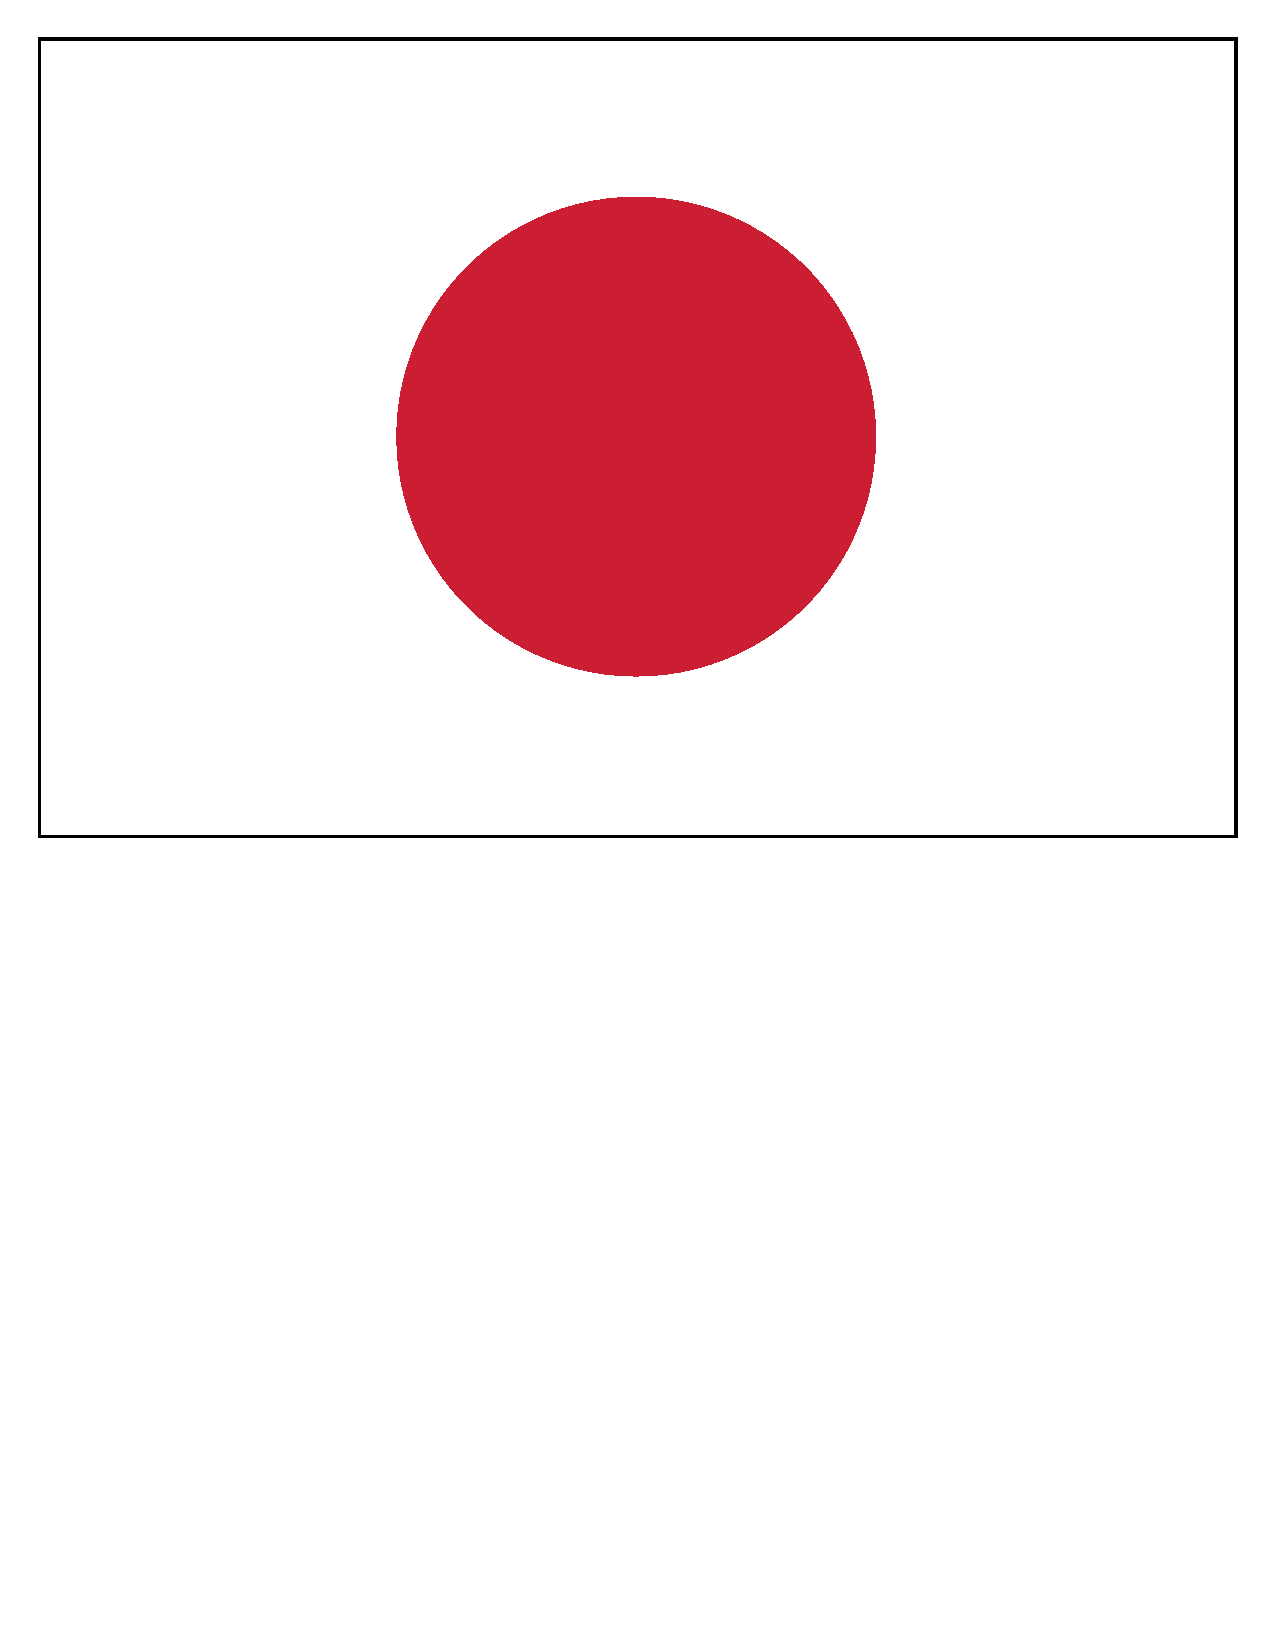
\includegraphics[width=0.4cm]{Images/Japan.pdf} Japanese (conversational)
	}

%!TEX root = ../todd-cv.tex
%----------------------------------------------------------------------------------
%            Software Projects
%----------------------------------------------------------------------------------
\section{Software Projects\see{\href{https://github.com/scalability-llnl}{github.com/scalability-llnl}}}
	\cvitem{\github{spack}}{
		Package manager/port system for HPC software.}
	\cvitem{cram}{
		Tool for running ensembles of millions of small MPI jobs.}
	\cvitem{\github{rubik}}{
		Tool for building optimized task mappings for structured simulation codes on supercomputers.}
	\cvitem{\github{callpath}}{
		Library for representing stack traces compactly in distributed applications.}
	\cvitem{\github{wrap}}{
		Generates interposition libraries to measure MPI applications.  Used in Allinea DDT.	}
	\cvitem{\github{muster}}{
		Scalable parallel clustering library, used in performance/debugging tools.}
	\cvitem{\github{nami}}{
		Parallel and sequential wavelet compression library.}
	\cvitem{\github{libra}}{
		Scalable load-balance measurement/viewer tool for MPI simulations.}
	\cvitem{\href{https://computation-rnd.llnl.gov/performance-analysis-through-visualization/software.php}{Boxfish}}{
		Visualization tool for performance data on torus networks.\hfill
	}


%----------------------------------------------------------------------------------
%            Publications
%----------------------------------------------------------------------------------
\section{Publications}
	% Compensate for bibliography's missing section header
	\renewcommand{\section}[1]{}
	\setlength{\presubspace}{.7em}
	\setlength{\postsubspace}{-.6em}

	\vspace{-.29in}

	\subsection{\paperSecTitle}
	\nocitePaper{*}
	\bibliographystylePaper{plain-url-inline-revchron}
	\bibliographyPaper{Bibliographies/Papers}
	
	\subsection{\workshopSecTitle}
	\nociteWorkshop{*}
	\bibliographystyleWorkshop{plain-url-inline-revchron}
	\bibliographyWorkshop{Bibliographies/Workshops}

	\subsection{\bookSecTitle}
	\nociteBook{*}
	\bibliographystyleBook{plain-url-inline-revchron}
	\bibliographyBook{Bibliographies/Books}

	\subsection{\phdSecTitle}
	\nocitePhD{*}
	\bibliographystylePhD{plain-url-inline-revchron}
	\bibliographyPhD{Bibliographies/PhD}	

	\subsection{\posterSecTitle}
	\nocitePoster{*}
	\bibliographystylePoster{plain-url-inline-revchron}
	\bibliographyPoster{Bibliographies/Posters}
		
\end{document}













